\documentclass[14pt,a4paper]{extarticle}
\usepackage[a4paper,top=12mm,bottom=12mm,left=14mm,right=14mm]{geometry}
\usepackage[T1]{fontenc}
\usepackage{amsmath}
\usepackage{amssymb}
% A sans serif font with a single-storey a, as children write it. It is
% used for the mathematics as well as the text.
\usepackage{tgadventor}
\renewcommand*{\familydefault}{\sfdefault}
\usepackage[italic]{mathastext}
\usepackage{xcolor}
\usepackage{array}
\usepackage{tikz}
\usepackage[most]{tcolorbox}
\usetikzlibrary{arrows.meta}

% ================================================================
% Always, sometimes or never: an extension to the algebraic terminology
% sheet, for a Year 7 class meeting algebra for the first time.
%
% The sheet teaches pupils to decide whether a statement about a
% variable is always, sometimes or never true, and to write the
% argument: an example where the statement is true, a counterexample
% where it is false, or a reason that works for every number. The idea
% it is built on is that one counterexample is enough to show that a
% statement is not always true, while examples that work can never show
% that it is always true. The worked examples say this as they go.
%
% Page 1 has a worked example that tests a statement with a whole
% number, a decimal and a negative number, and Q1 is the same layout
% with gaps.
%
% Page 2 has the same layout with fewer gaps, where pupils choose their
% own values (Q2). Then a worked example gives a counterexample to an
% "every" statement, and Q3 gives counterexamples to statements about
% the words from the terminology sheet.
%
% Page 3 has a worked example that gives a reason for a statement that
% is always true. Q4 mixes always, sometimes and never, Q5 asks why ten
% examples do not show "always", and Q6 is open.
%
% The sheet is A4 in 14pt type, so that it can also be printed at A5
% (the type is then about 10pt). The answers are in a comment beside
% each question.
% ================================================================

\pagestyle{empty}
\setlength{\parindent}{0pt}
\setlength{\parskip}{0pt}
% Ragged right, so that the spaces between words are all the same.
\AtBeginDocument{\raggedright}

% The idea the sheet is built on, and the worked examples, in boxes that
% are tinted only faintly, so that the sheet is cheap to print.
\newtcolorbox{keyidea}{colback=orange!3,colframe=orange!35,boxrule=0.6pt,
  left=6pt,right=6pt,top=4pt,bottom=4pt,before upper=\raggedright}
\newtcolorbox{wex}[1]{colback=blue!2,colframe=blue!30,boxrule=0.6pt,
  colbacktitle=blue!8,coltitle=blue!50!black,
  left=6pt,right=6pt,top=3pt,bottom=4pt,before upper=\raggedright,
  title={\bfseries Worked example: #1},
  toptitle=1pt,bottomtitle=1pt}

% A question number, and gaps to write in: \gap for a number or a term,
% and \wgap for a word or an expression. The strut keeps the lines far
% enough apart to write on at A5.
\newcommand{\qn}[1]{\textbf{Q#1.}\ }
\newcommand{\gapstrut}{\rule[-1.5mm]{0pt}{7.5mm}}
\newcommand{\gap}{\gapstrut\underline{\hspace{1.4cm}}}
\newcommand{\wgap}{\gapstrut\underline{\hspace{3.4cm}}}

% A line to write a sentence on, the full width of the text.
\newcommand{\writeline}{\par\gapstrut\underline{\hspace{\linewidth}}\par}

% A statement to decide about.
\newcommand{\statement}[1]{\textbf{Statement:} #1\par}

% The table for testing a statement with values of x, and the sentences
% about it beside it. Each row of the table is tall enough to write in
% at A5.
\newcolumntype{C}[1]{>{\centering\arraybackslash}p{#1}}
\newcommand{\rowstrut}{\rule[-2.6mm]{0pt}{8.4mm}}
\newenvironment{testtable}[2]
  {\begin{minipage}[t]{7cm}\vspace{0pt}%
   \renewcommand{\arraystretch}{1.1}%
   \begin{tabular}{|C{1.3cm}|C{1.5cm}|C{2.8cm}|}\hline
   $x$ & #1 & #2\\ \hline}
  {\end{tabular}\end{minipage}}
\newenvironment{sentences}
  {\begin{minipage}[t]{0.56\linewidth}\vspace{0pt}\raggedright}
  {\end{minipage}}

% The three answers to circle, at the right-hand end of the line.
\newcommand{\circleone}{\hfill always\qquad sometimes\qquad never\par}

\begin{document}

% ================================================================
% PAGE 1: testing a statement with numbers
% ================================================================

\begin{center}
  {\LARGE\bfseries Always, Sometimes or Never?}
\end{center}
\vspace{-4pt}

\begin{keyidea}
\centering
A statement can be \textbf{always true}, \textbf{sometimes true} or
\textbf{never true}.
\end{keyidea}

\vspace{10pt}
\begin{wex}{a statement that is sometimes true}
\statement{$2x$ is bigger than $x$.}
We test the statement with a whole number, a decimal and a negative
number.

\vspace{6pt}
\begin{testtable}{$2x$}{Is $2x$ bigger than $x$?}
  \rowstrut $3$   & $6$  & yes\\ \hline
  \rowstrut $0.5$ & $1$  & yes\\ \hline
  \rowstrut $-1$  & $-2$ & no\\ \hline
\end{testtable}\hfill
\begin{sentences}
When $x=3$, $2x=6$, which is bigger than $3$. So the statement is true
when $x=3$.

\vspace{6pt}
When $x=-1$, $2x=-2$, which is smaller than $-1$. So $x=-1$ is a
\textbf{counterexample}: the statement is false when $x=-1$.

\vspace{6pt}
The statement is true for some values of $x$ and false for others, so
it is \textbf{sometimes true}.
\end{sentences}
\end{wex}

\vfill
% Answers: the table is 9, yes; 0.25, no; 4, yes. The gaps are 9;
% true; 0.25; counterexample; false; sometimes.
\qn{1} Complete the table and the sentences.

\vspace{4pt}
\statement{$x^2$ is bigger than $x$.}
\vspace{6pt}
\begin{testtable}{$x^2$}{Is $x^2$ bigger than $x$?}
  \rowstrut $3$   & & \\ \hline
  \rowstrut $0.5$ & & \\ \hline
  \rowstrut $-2$  & & \\ \hline
\end{testtable}\hfill
\begin{sentences}
When $x=3$, $x^2=$ \gap, which is bigger than $3$. So the statement is
\wgap\ when $x=3$.

When $x=0.5$, $x^2=$ \gap, which is smaller than $0.5$. So $x=0.5$ is
a \wgap: the statement is \wgap\ when $x=0.5$.

The statement is true for some values of $x$ and false for others, so
it is \wgap\ true.
\end{sentences}
\vfill

\newpage
% ================================================================
% PAGE 2: counterexamples to "every" statements, and choosing values
% ================================================================

% Answers: open. The statement is true for every positive x, for
% example x = 4 gives 10 - x = 6. A counterexample is 0 or any negative
% number, for example x = -2 gives 10 - x = 12. It is sometimes true.
\qn{2} Choose three values of $x$ to test, including a negative number.
Then complete the sentences.

\vspace{4pt}
\statement{$10-x$ is smaller than $10$.}
\vspace{6pt}
\begin{testtable}{$10-x$}{Is $10-x$ smaller than $10$?}
  \rowstrut & & \\ \hline
  \rowstrut & & \\ \hline
  \rowstrut & & \\ \hline
\end{testtable}\hfill
\begin{sentences}
When $x=$ \gap, $10-x=$ \gap, so the statement is true.

When $x=$ \gap, $10-x=$ \gap, so $x=$ \gap\ is a \wgap.

The statement is \wgap\ true.
\end{sentences}

\vfill
\begin{wex}{a counterexample to an ``every'' statement}
\statement{Every term has a coefficient that is a whole number.}
The term $0.5a$ has the coefficient $0.5$, which is not a whole number.
So $0.5a$ is a counterexample, and the statement is false. One
counterexample is enough: we do not need to look at any other terms.
\end{wex}

\vfill
\qn{3} Each statement is false. Fill in the gaps to give a
counterexample.

\vspace{6pt}
% Answer: open. Any expression whose terms all have a variable, for
% example 4x + y.
(a) \textit{Every expression has a constant.}\par
The expression \wgap\ has no constant. So the statement is false.

\vspace{8pt}
% Answers: 3 terms; 2 variables.
(b) \textit{Every expression with $3$ terms has $3$ variables.}\par
The expression $2a+3b+1$ has \gap\ terms, but only \gap\ variables.
So the statement is false.

\vspace{8pt}
% Answers: open. Any negative value of x, for example x = -2 gives 6.
(c) \textit{The term $-3x$ always has a negative value.}\par
When $x=$ \gap, the term $-3x$ has the value \gap, which is not
negative. So the statement is false.

\vspace{8pt}
% Answers: open. For example the term x, which has the coefficient 1,
% or 0.5a, which has the coefficient 0.5.
(d) \textit{Every term has a coefficient bigger than $1$.}\par
The term \gap\ has the coefficient \gap, which is not bigger than $1$.
So the statement is false.
\vfill

\newpage
% ================================================================
% PAGE 3: reasons, mixed statements, and open questions
% ================================================================

\begin{wex}{a statement that is always true}
\begin{minipage}[t]{0.55\linewidth}
\vspace{0pt}\raggedright
\statement{$x+3$ is bigger than $x$.}
Testing cannot show this, because we cannot test every number. Instead
we give a reason: adding $3$ to a number moves it $3$ to the right on
the number line, and a number further to the right is bigger. So $x+3$
is bigger than $x$ for every value of $x$, and the statement is
\textbf{always true}.
\end{minipage}\hfill
\begin{minipage}[t]{0.42\linewidth}
\vspace{14pt}
\centering
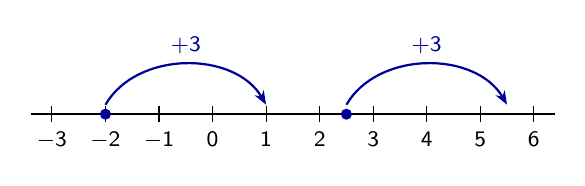
\begin{tikzpicture}[x=0.68cm]
  \draw[thick] (-3.4,0) -- (6.4,0);
  \foreach \v in {-3,...,6} {
    \draw (\v,-0.1) -- (\v,0.1);
    \node[below, font=\footnotesize] at (\v,-0.1) {$\v$};
  }
  % two of the jumps of +3, from a negative number and from a decimal
  \foreach \a in {-2, 2.5} {
    \fill[blue!60!black] (\a,0) circle (2pt);
    \draw[-{Stealth[length=5pt]}, thick, blue!60!black]
      (\a,0.12) to[out=60, in=120]
      node[above, font=\footnotesize] {$+3$} ({\a+3},0.12);
  }
\end{tikzpicture}
\end{minipage}

\vspace{6pt}
In the same way, $x-4$ is \textbf{never} bigger than $x$, because
subtracting $4$ moves a number $4$ to the left.
\end{wex}

\vfill
\qn{4} Circle always, sometimes or never. Then write an example and a
counterexample, or a reason.

\vspace{6pt}
% Answer: always. x + x is two lots of x, which is 2x.
(a) $x+x=2x$ \circleone
\writeline

\vspace{6pt}
% Answer: sometimes. True when x = 5 (both are 0). False when x = 0:
% 5 - x = 5 but x - 5 = -5.
(b) $5-x$ and $x-5$ have the same value. \circleone
\writeline

\vspace{6pt}
% Answer: never. x^2 is x multiplied by itself, and a positive number
% times a positive number, or a negative number times a negative number,
% is positive. 0^2 = 0, which is not negative.
(c) $x^2$ is negative. \circleone
\writeline

\vspace{6pt}
% Answer: sometimes. True when x = 4 (2 is smaller than 4). False when
% x = -4 (-2 is bigger than -4), or when x = 0.
(d) $\dfrac{x}{2}$ is smaller than $x$. \circleone
\writeline

\vfill
% Answer: ten values that work cannot show that the statement is true
% for every value. Counterexamples: x = 0 (3x = 0, x + 1 = 1),
% x = 0.5 (both are 1.5), or any negative number.
\qn{5} Sam tests the statement ``$3x$ is bigger than $x+1$'' with
$x=1, 2, 3, \dots, 10$. It is true every time, so Sam says that the
statement is always true. Explain why Sam is wrong.
\writeline
A counterexample is $x=$ \gap, because $3x=$ \gap\ and $x+1=$ \gap.

\vfill
% Answer: open. For example "x + 2 is bigger than 5" is true when
% x = 4 and false when x = 1.
\qn{6} Write your own statement about $x$ that is sometimes true. Give a
value of $x$ that makes it true, and a counterexample.
\writeline
\writeline
\vfill

\end{document}
